\chapter{Successful NoSQL case studies}

To support our proposal of implementing a NoSQL system, we present in this section some successful case studies which show that selecting such a new alternative (in comparison with the consolidated systems) to the classic RDBMS in big scientific projects is more than a risk, the main reason argued by NoSQL detractors.


\section{CMS at the LHC: MongoDB}

High-energy physicists working at the Compact Muon Solenoid (CMS) detector at the LHC, that generates more than 100 datacentres in a three-tier model and generates around 10PB of data each year, are benefiting from a NoSQL database management system that gives them unified access to data from a huge variety of sources (from relational and non-relational data sources, such as relational databases, document-oriented databases, blogs, wikis, file systems and customised applications). The team providing data management to the CMS Cern project has built a system using MongoDB in preference to relational database technologies and other non-relational options. The reasons to select MongoDB were:

\begin{itemize}
\item Dynamic queries support
\item Full indexes
\item Auto-sharding
\end{itemize}

Several years ago the data management group at the CMS confronted a data discovery problem, with a variety of databases necessitating a user interface that would hide the complexity of the underlying architecture from the physicists. There was a vast variety of distributed databases and different formats (HTML, XML, JSON files, etc.).

To provide the ability to search and aggregate information across this complex data landscape CMS's Data Management and Workflow Management (DMWM) project created a data aggregation system (DAS), built on MongoDB.  According to Valentin Kuznetsov, a research associate at Cornell University, and team member, ``there was nothing specific to the system related to our experiment'', so it can be deduced that this MongoDB approach is extensible. 




\section{ATLAS Workload Management System: Cassandra}

A Thoroidal LHC Apparatus (ATLAS) is another of the six particle detectors experiments at LHC at CERN, whose data handling is a real challenge: almost 1 billion proton proton interactions per second leading to more than 10PBytes per year (it actually generates 1PByte of raw data each second, before filtering). By 2014, the expected data rate will be 40 PBytes per year.

% \begin{figure}[tb]
% \centering
% 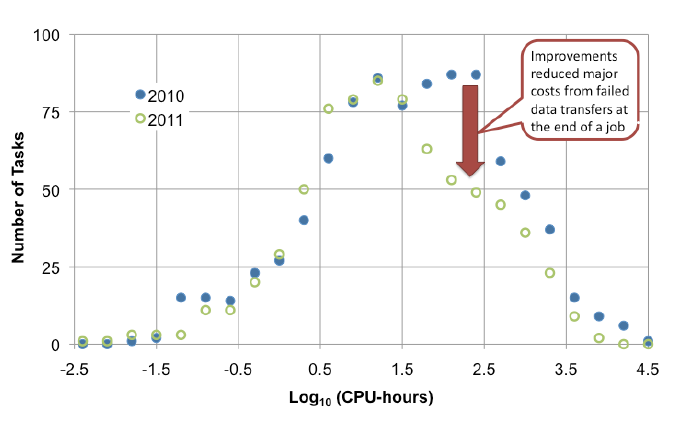
\includegraphics[width=14cm,height=8cm]{images/panda.png}
% \caption{Weibull distribution of CPU-hours used to recover job failures in petascale data processing, from \href{https://sharepoint.anl.gov/hep/HEP\%20Accomplishments/Highlights_101212.pdf}{Argonne National Laboratory}}
% \end{figure}

The reason to select a NoSQL solution is there is no need to store the monitoring data in a RDBMS, deciding instead a system which can provide a very high degrees of availability, resilience and scalability.

At first stage, two of the most popular platforms were considered: Apache Cassandra \footnote{More information in \href{http://cassandra.apache.org/}{Apache Cassandra Website}} and Apache Hbase. As Cassandra has a lower learning curve, and considering that it was already deployed in ATLAS, the decision was done.

As a matter of fact, in the tests done, Cassandra's time per extracted entry was 10 ms, with 10 concurrent clients. This means 1000 queries per second, about twice the rate currently experienced by their Oracle DB. An analogous test done against Oracle (from a Python client) yielded roughly 100ms per query. \footnote{More information at \href{http://cds.cern.ch/record/1446655/files/ATL-SOFT-PROC-2012-012.pdf}{CERN Document Center}.}


\section{Measuring radiation levels in Seattle: Cloudant}

Researchers at the University of Washington used the Cloudant \footnote{See \href{https://cloudant.com/}{Cloudant Website}} database as part of an experiment that determined radiation levels in Seattle as a result of the recent Fukushima nuclear disaster are ``well below alarming limits.`` The research team, which includes Cloudant Founder and Chief Scientist Mike Miller studied particles captured from the five air filters and used Cloudant’s CouchDB-based BigCouch database to store and process the data. They chose Cloudant because with it, it was possible to start monitoring radiation levels very quickly, after a very easy setup and the capability of sampling gigantic quantities of air, allowing them to analyze the data and sharing it in near-real-time, profiting from BigCouch MapReduce engine.
